\chapter{实验和结论}\label{ch:exp}

本章将通过模拟数据和真实数据,验证本文提出的增量式集束调整框架的通用性,以及测试本文算法和传统批量式集束调整算法(基于Ceres-Solver)的速度和精度。Ceres-Solver是SLAM系统中常用的非线性最小二乘求解器,提供了稠密版本和稀疏版本的多种批量式数值优化算法实现(包括LM方法、DL法等),且具有较好的数值稳定性和效率。

\section{通用问题测试}

本文提出的框架具备较好的通用性,除了能求解视觉惯性SLAM的集束调整问题,也能求解一般的非线性最小二乘问题。本节将通过求解一个简单的曲线拟合的示例验证通用性。

\subsection{测试设置}

\begin{figure}[htb!]
    \centering
    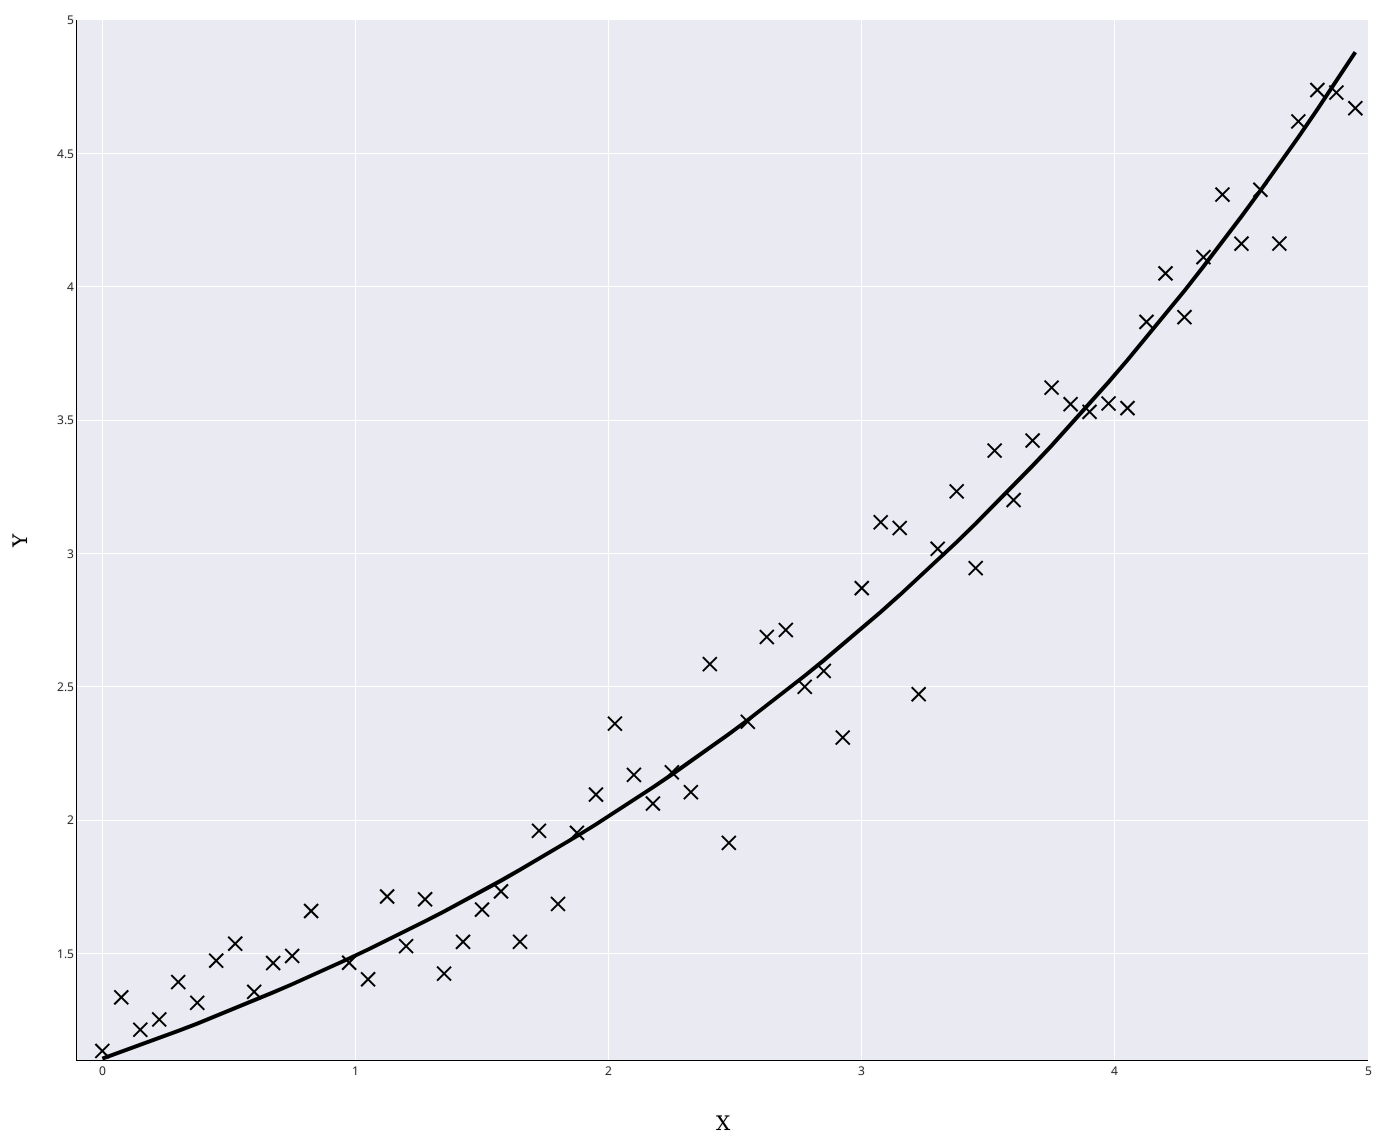
\includegraphics[width=.65\textwidth]{Pictures/curse_fitting_gt.png}
    \caption{曲线拟合问题:输入散点图和真值曲线}
    \label{fig:curve_gt}
\end{figure}

测试问题为曲线拟合问题:
\begin{equation}
    y = e^{mx+c}
\end{equation}
其中$(x,y)$为输入数据集,$m$和$c$为曲线待估参数,使用最小二乘拟合曲线。使用参数$m=0.3,c=0.1$生成真值曲线$y=e^{0.3x+0.1}$,并在真值曲线上增加高斯噪声:$n\sim\mathcal{N}(0,0.2^2)$,获得输入数据。如图~\ref{fig:curve_gt}展示了输入数据的散点图和对应的真值曲线。

\subsection{结果对比}

使用Ceres-Solver和本文的集束调整框架进行求解,其中Ceres-Solver的非线性求解策略选取LM法,本文的优化策略为HLMDL法,并将两者的初始阻尼因子均设置为$1.0$,初始参数值均设置为$m=0.0,c=0.0$,对比曲线拟合的结果。

\begin{figure}[htb!]
    \centering
    \subfloat[Ceres-LM:曲线拟合结果]{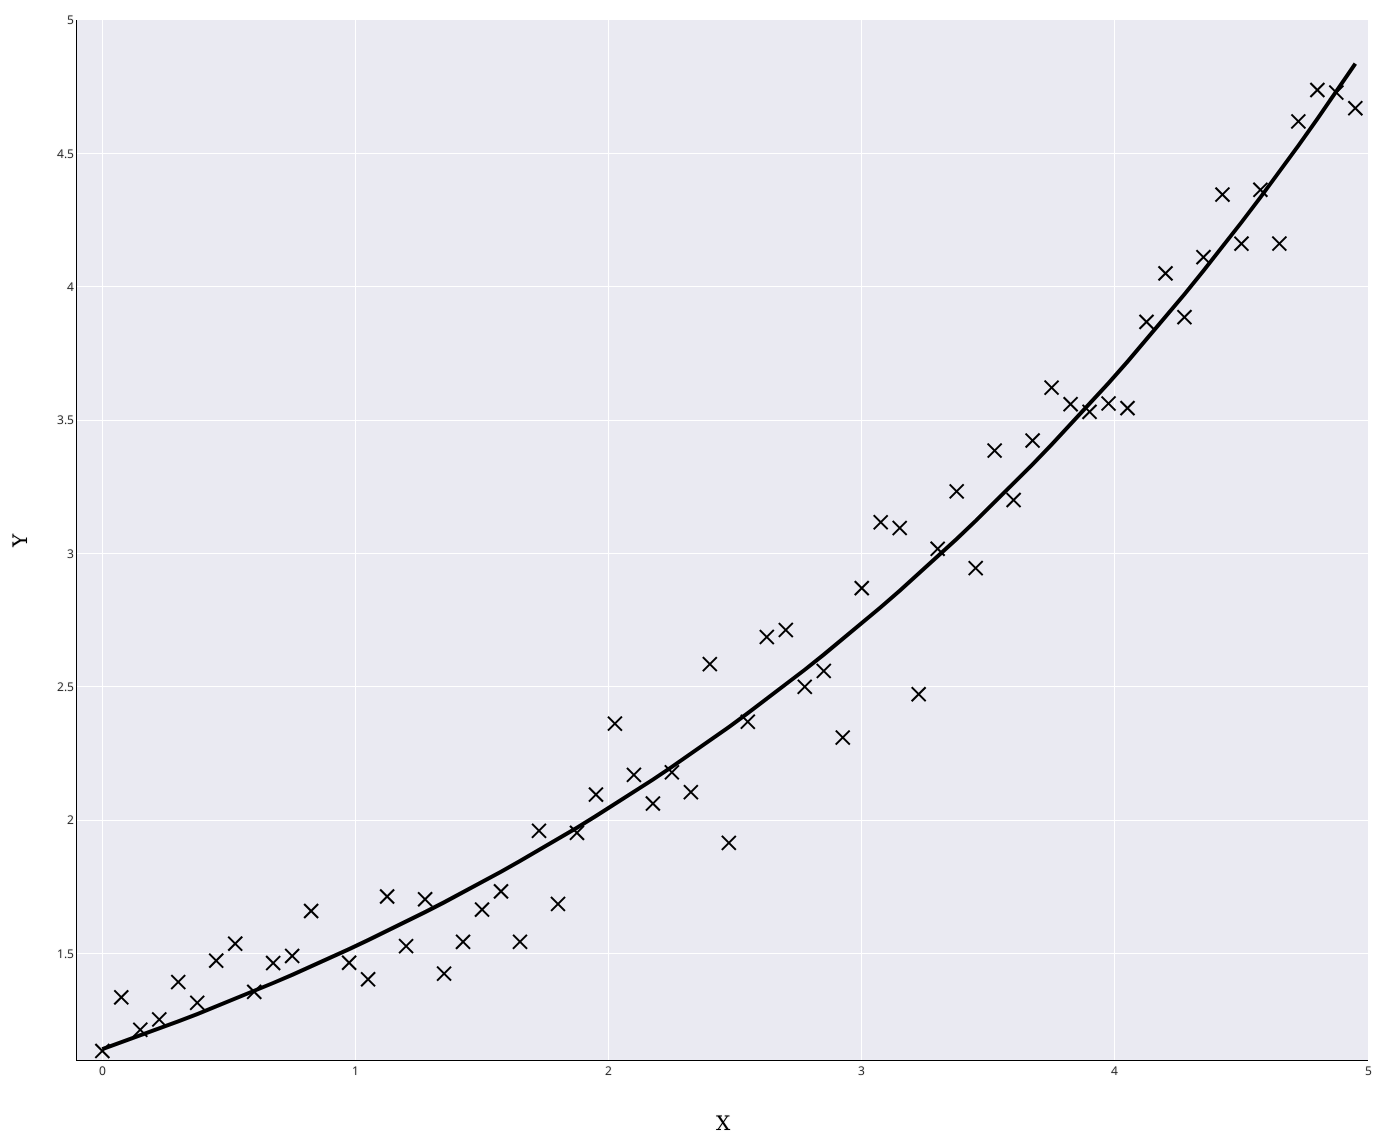
\includegraphics[width=.48\textwidth]{Pictures/curse_fitting_ceres.png}}~
    \subfloat[HLMDL:曲线拟合结果]{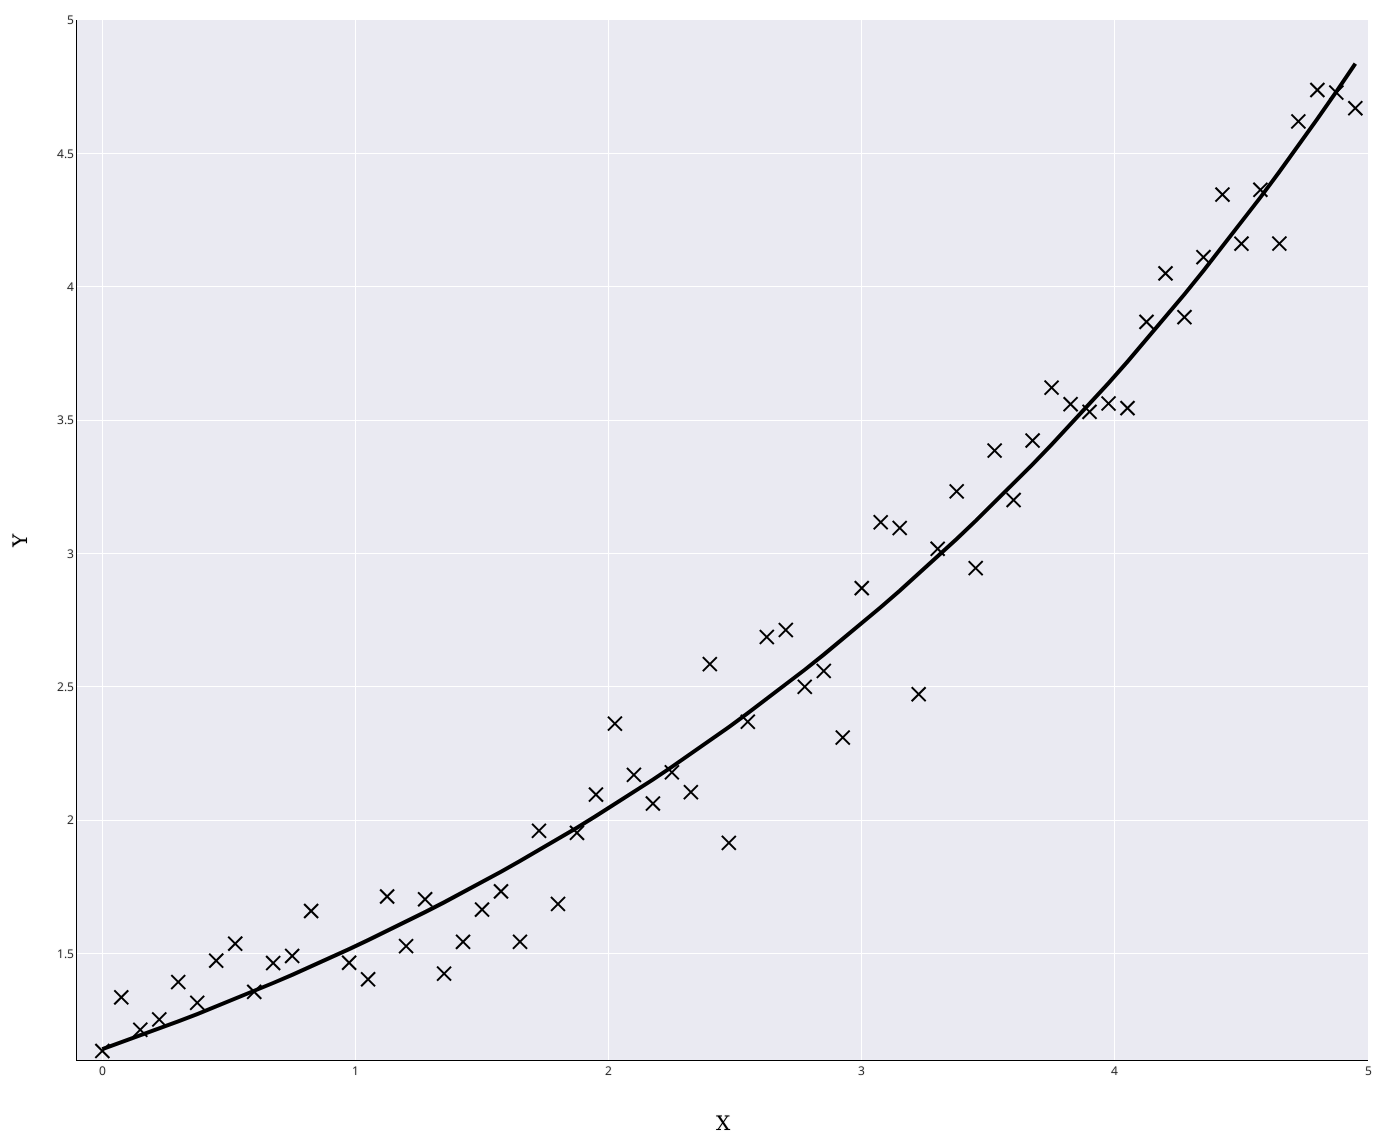
\includegraphics[width=.48\textwidth]{Pictures/curse_fitting_spec3.png}}
    \caption{曲线拟合运行结果:左图为Ceres-LM求解所得的拟合曲线,右图为HLMDL求解所得的拟合曲线}
    \label{fig:curve}
\end{figure}

经过迭代,Ceres-Solver解得参数$m=0.291865,c=0.131423$,本文的HLMDL解得参数$m=0.291871,c=0.131401$,两者均可收敛到真值附近。图~\ref{fig:curve}展示了两者算法的结果,可见本文提出的集束调整框架也支持求解一般的最小二乘问题,具备较好的通用性。

\section{集束调整测试}

本节将通过求解模拟集束调整问题和真实集束调整问题来验证本文提出的集束调整框架的速度和精度。

\subsection{测试设置}

测试数据包含本文自行模拟生成的相机-IMU-三维点的数据集Cubic-50和包含相机-三维点的VSLAM真实数据集Cathedral\citep{kim2014influence}和Venice\citep{kummerle2011g}。其中Cubic-50数据集为模拟生成的带高斯噪声的VISLAM数据集,包含IMU预积分的结果和协方差、相机状态的初值、视觉观测。Cathedral和Venice为真实数据集,包含相机状态的初值、三维点状态的初值和视觉观测。这样的设置省去了SLAM前端视觉匹配、IMU积分的过程,保证所有算法求解的问题相同。几组数据具体包含的内容如表~\ref{tab:dataset}所示,由于Ceres-Solver的DL法策略求解完整的Cathedral数据集和Venice数据集失败,即集束调整求解过程中能量不能收敛,顾只取Cathedral数据集的前$45$个相机状态,和Venice数据集的前$50$个相机状态,后文将用Cathedral-46和Venice-51代表这两个数据集。

{
\linespread{1}
\begin{table}[htb!]
\zihao{5}
\caption{测试数据集明细}
\label{tab:dataset}
\centering
\begin{tabular}{l|cccc}
    \toprule
    数据集       & 相机数量 & 三维点数量 & IMU目标函数数量 & 重投影误差目标函数数量 \\ \midrule
    Cubic-50     &       50 &        163 &              49 &                    789 \\
    Venice-51    &       51 &      35110 &               0 &                 117988 \\
    Cathedral-46 &       46 &      33717 &               0 &                 208079 \\
    \bottomrule
\end{tabular}
\end{table}
}

所有测试均基于最新的Arch Linux操作系统,搭载主频为3.6GHz的Intel Core i7-7700处理器,内存为8GB。运行测试期间关闭其他所有应用程序,每一组测试的结果均取10次运行后的平均值。

\subsection{结果对比}

为了保证公平,所有求解器尽可能地设置成相同的算法,并将算法运行时间$T$定义为从问题构建开始到完成求解的总时间。所有优化器均使用稀疏求解策略,本文的优化策略非线性部分为HLMDL法,线性部分为增量舒尔补-Cholesky分解和增量舒尔补I-PCG迭代法。Ceres-Solver的非线性优化策略则选取LM法和DL法,线性部分设置为舒尔补-QR分解法。将所有优化算法的迭代次数设置为相同,通过对比运行时间$T$和迭代次数$t$来比较不同的求解策略的效率。通过对比求解结束时的总能量,即重投影误差目标函数的值$E_{\text{proj}}$和IMU预积分目标函数的值$E_{\text{IMU}}$来对比精度。

表~\ref{tab:time}展示了时间测试对比结果,包含运行时间、总的迭代次数以及每条实例耗时相对于测试基准耗时的百分比,并将第一行设置为其他测试实例的对比基准。例如第一行代表的是Ceres-Solver的DL法运行结果,使用的非线性策略为DL法,线性策略为舒尔补和QR分解,在Cubic-50数据集上求解共进行$5$次迭代,平均耗时$69$毫秒,相对于基准耗时的百分比为$100\%$。

{
\linespread{1}
\begin{table}[htb!]
\zihao{5}
\caption{测试结果:运行时间和迭代次数}
\label{tab:time}
\centering
\begin{tabular}[b]{l|ccc}
    \toprule
    求解策略耗时(T/t)       &   Cubic-50 &       Venice-51 &    Cathedral-46 \\ \midrule
    Ceres-LM:Schur-QR        & $48$ms/$4$ & $23018$ms/$230$ & $42706$ms/$204$ \\
    耗时相对于基准的百分比    &  $100.0\%$ &       $100.0\%$ &       $100.0\%$ \\ \midrule
    Ceres-DL:Schur-QR        & $44$ms/$4$ &            失败 &            失败 \\
    耗时相对于基准的百分比    &   $91.7\%$ &             N/A &             N/A \\ \midrule
    HLMDL:增量Schur-Cholesky & $17$ms/$4$ &  $4545$ms/$230$ &  $7924$ms/$204$ \\
    耗时相对于基准的百分比    &   $35.4\%$ &        $19.7\%$ &        $18.6\%$ \\ \midrule
    HLMDL:增量Schur-I-PCG    & $18$ms/$4$ &            失败 &  $6710$ms/$205$ \\
    耗时相对于基准的百分比    &   $37.5\%$ &             N/A &        $15.7\%$ \\
    \bottomrule
\end{tabular}
\end{table}
}

表~\ref{tab:energy}展示了精度测试对比结果,每个数据集的初始总能量和求解结束收敛时的总能量。

{
\linespread{1}
\begin{table}[htb!]
\zihao{5}
\caption{测试结果:收敛时的误差}
\label{tab:energy}
\centering
\begin{tabular}[b]{l|ccc}
    \toprule
    求解策略及收敛时总能量$E$ &          Cubic-50 &            Venice-51 &         Cathedral-46 \\
    总能量初始值$E_0$         & $2.514\times10^3$ &  $9.171\times10^{0}$ &  $3.600\times10^{0}$ \\ \midrule
    Ceres-LM:Schur-QR        & $4.956\times10^2$ & $1.599\times10^{-1}$ & $7.135\times10^{-1}$ \\
    Ceres-DL:Schur-QR        & $5.153\times10^2$ &                  N/A &                  N/A \\
    HLMDL:增量Schur-Cholesky & $4.982\times10^2$ & $2.045\times10^{-1}$ & $6.111\times10^{-1}$ \\
    HLMDL:增量Schur-I-PCG    & $5.004\times10^2$ &                  N/A &  $2.064\times10^{0}$ \\
    \bottomrule
\end{tabular}
\end{table}
}

表~\ref{tab:time}和表~\ref{tab:energy}中,“失败”或“N/A”项代表某求解策略在该数据集上能量无法收敛,相关数据无法提供。

图~\ref{fig:cubic}、图~\ref{fig:venice}和图~\ref{fig:cathedral}分别为使用Ceres-Solver和本文的增量式集束调整框架求解三个数据集所得的点云结果,可以看到,在Cubic-50数据集上,解得的点云质量没有显著差异;在Venice-51数据集上,使用本文提出的HLMDL-增量舒尔补算法解得的点云质量略好于Ceres-Solver解得的点云;而在Cathedral-46数据集上,本文提出的HLMDL-增量舒尔补算法解得的点云质量则要明显好于使用Ceres-Solver解得的点云。

\begin{figure}[htb!]
    \centering
    \subfloat[Ceres-LM:Cubic-50点云]{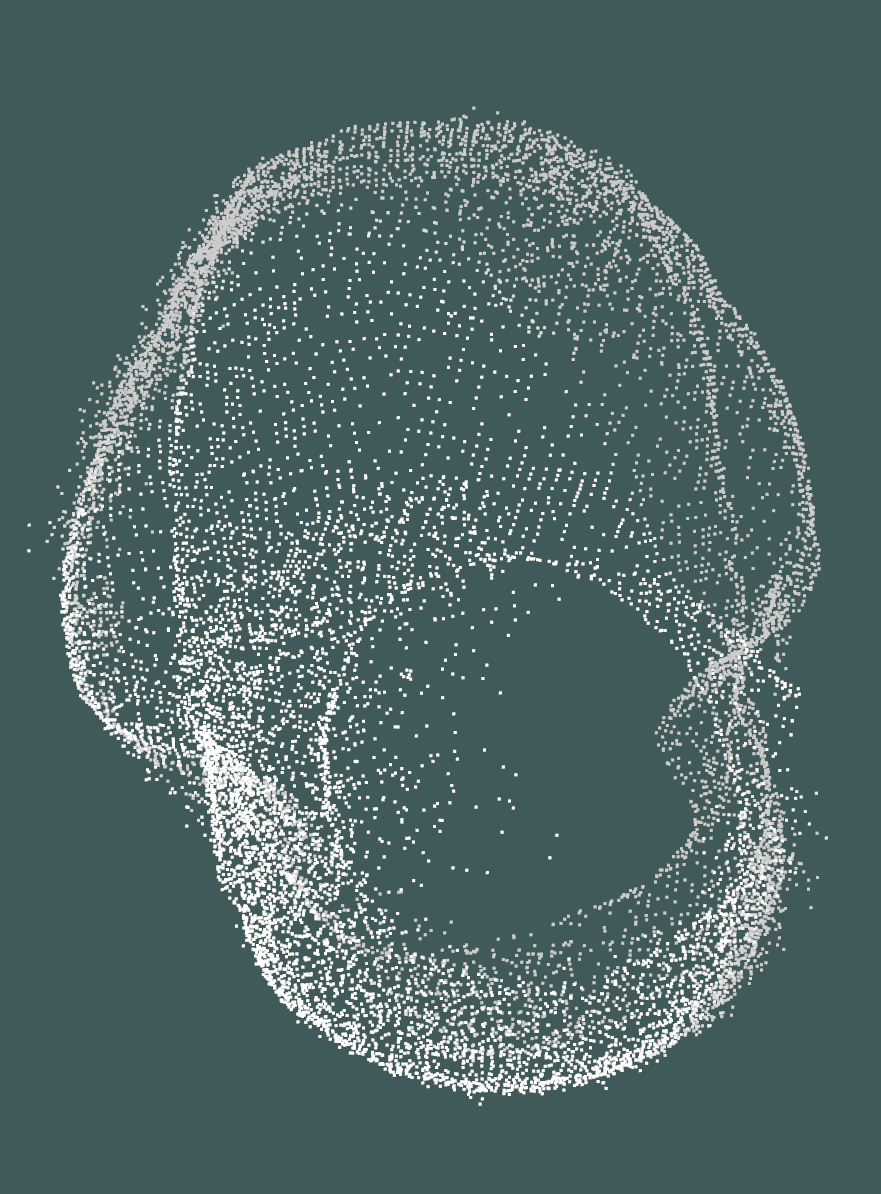
\includegraphics[width=.48\textwidth]{Pictures/cubic_ceres.png}}~
    \subfloat[HLMDL:Cubic-50点云]{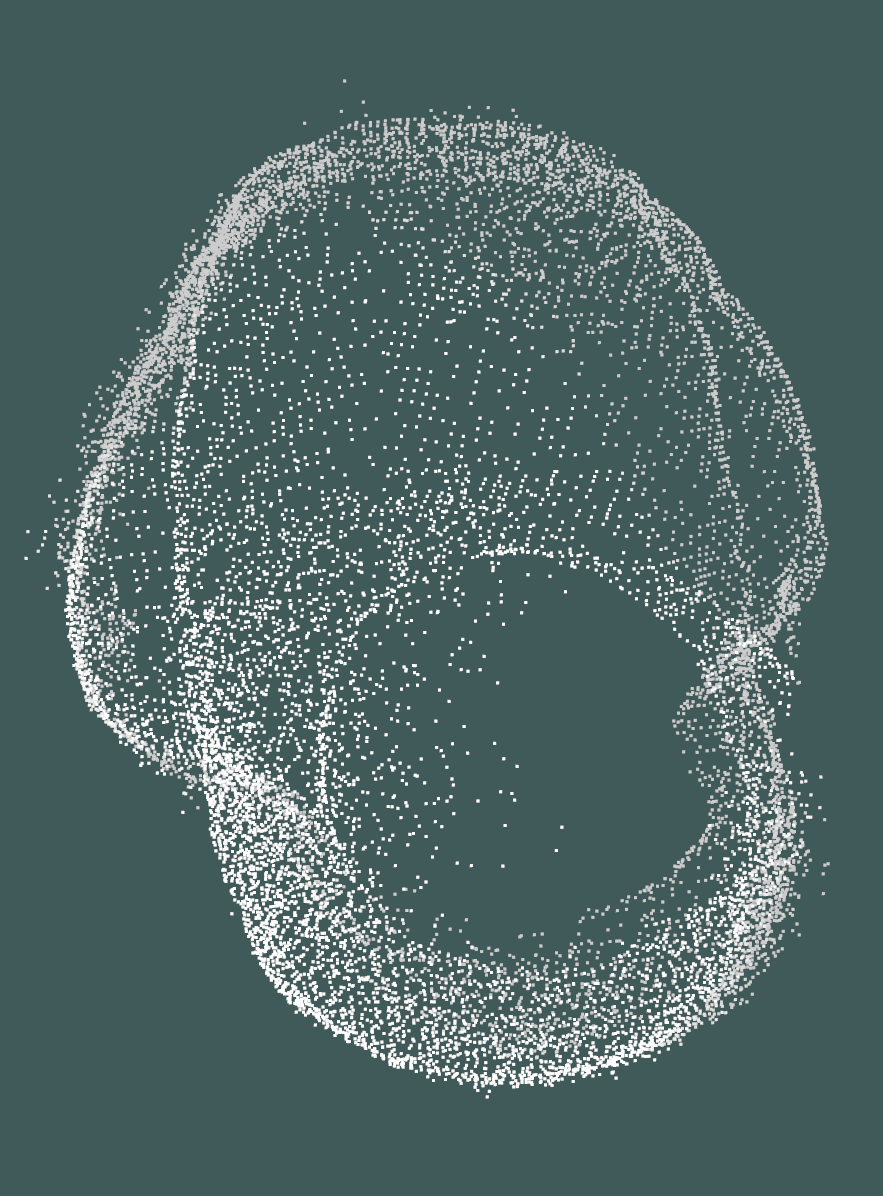
\includegraphics[width=.48\textwidth]{Pictures/cubic_spec3.png}}
    \caption{Cubic-50运行结果:左图为Ceres-LM求解所得的点云,右图为HLMDL求解所得的点云}
    \label{fig:cubic}
\end{figure}

\begin{figure}[htb!]
    \centering
    \subfloat[Ceres-LM:Venice-51正视图]{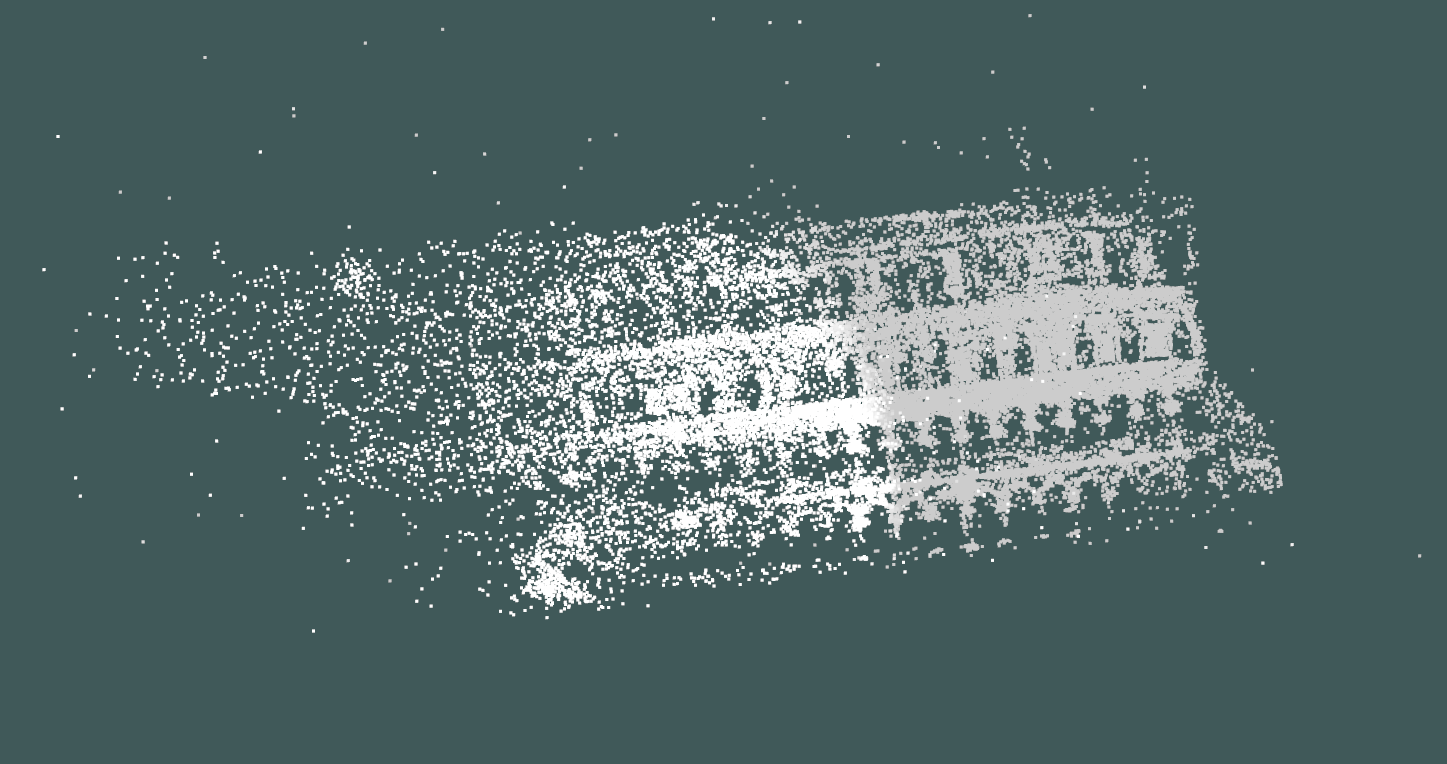
\includegraphics[width=.48\textwidth]{Pictures/venice_ceres.png}}~
    \subfloat[HLMDL:Venice-51正视图]{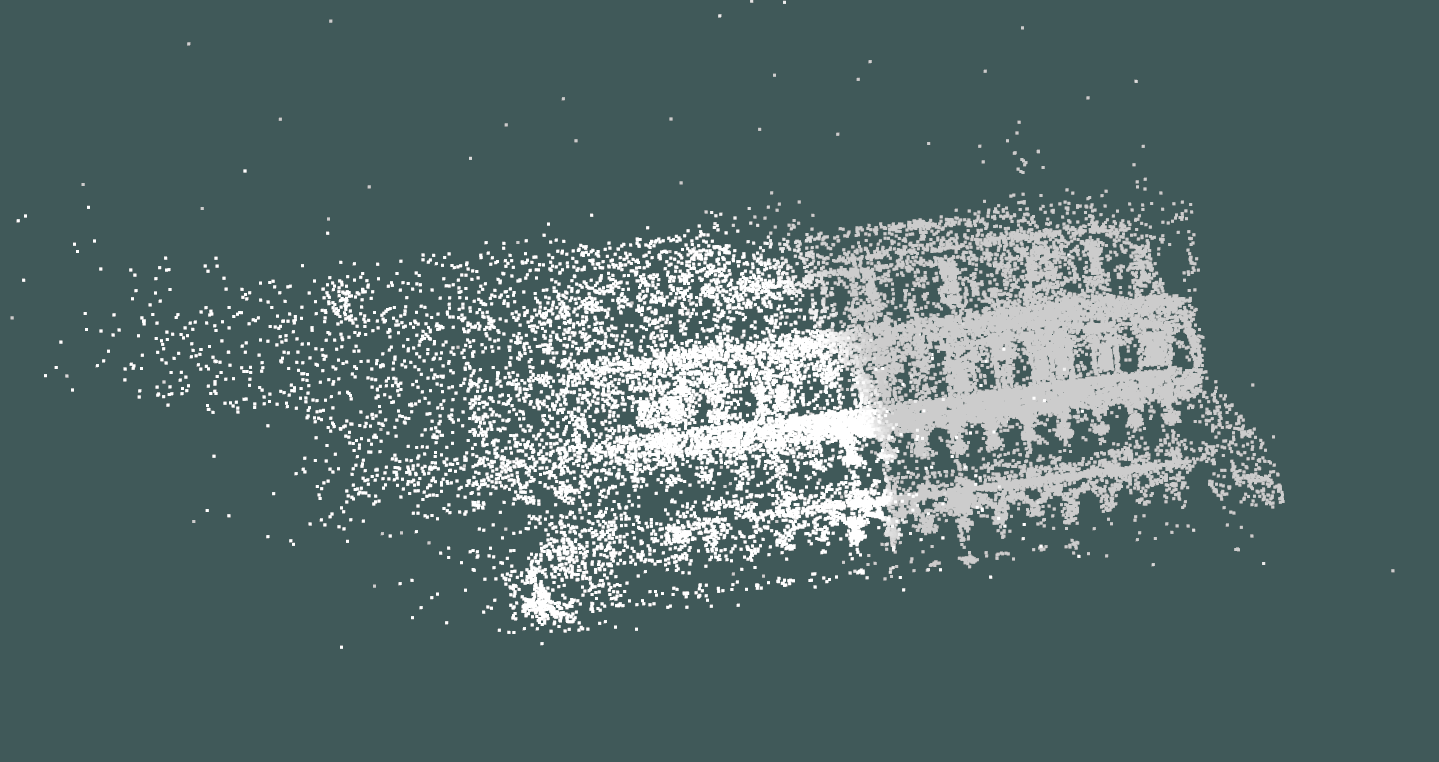
\includegraphics[width=.48\textwidth]{Pictures/venice_spec3.png}}
    \\
    \subfloat[Ceres-LM:Venice-51俯视图]{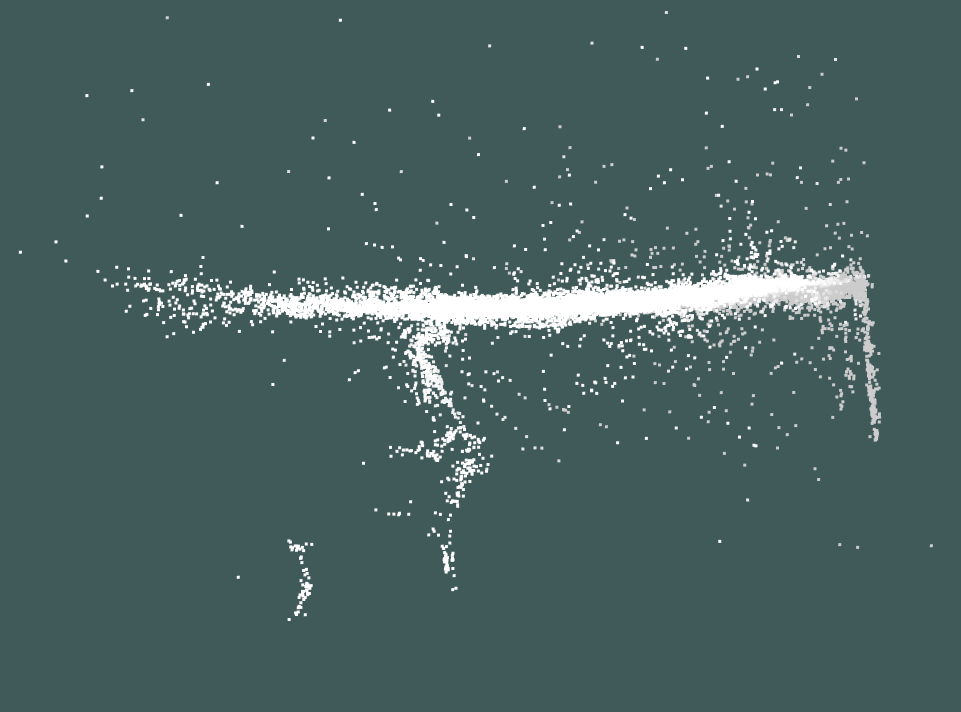
\includegraphics[width=.48\textwidth]{Pictures/venice_ceres_up.png}}~
    \subfloat[HLMDL:Venice-51俯视图]{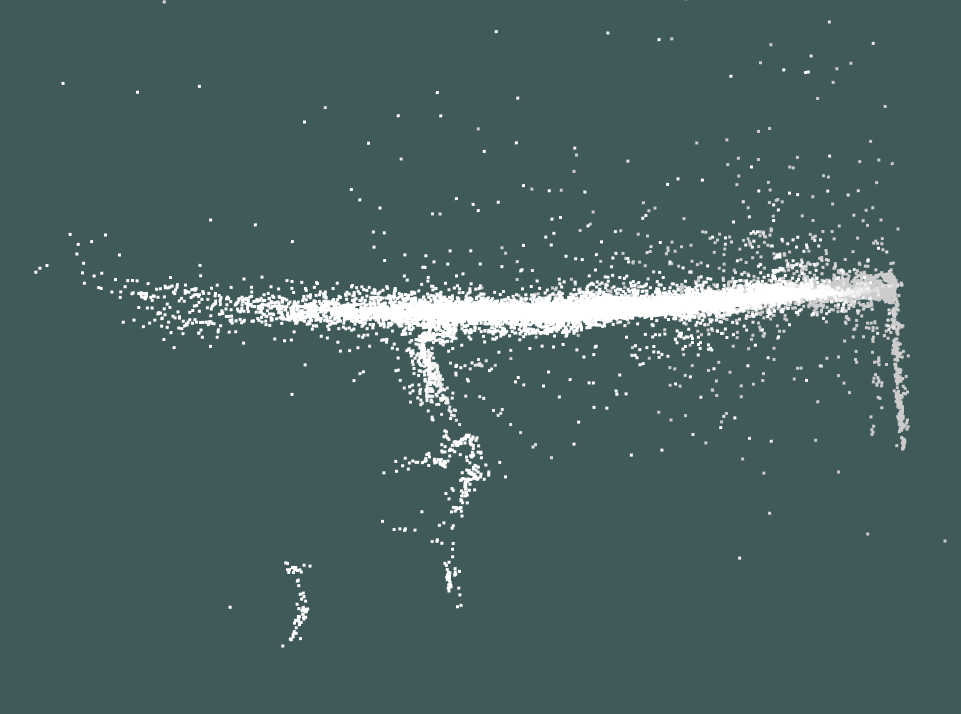
\includegraphics[width=.48\textwidth]{Pictures/venice_spec3_up.png}}
    \caption{数据集Venice-51运行结果:左列为Ceres-LM求解所得的点云,右列为HLMDL求解所得的点云}
    \label{fig:venice}
\end{figure}

\begin{figure}[htb!]
    \subfloat[Ceres-LM:Cathedral-46正视图]{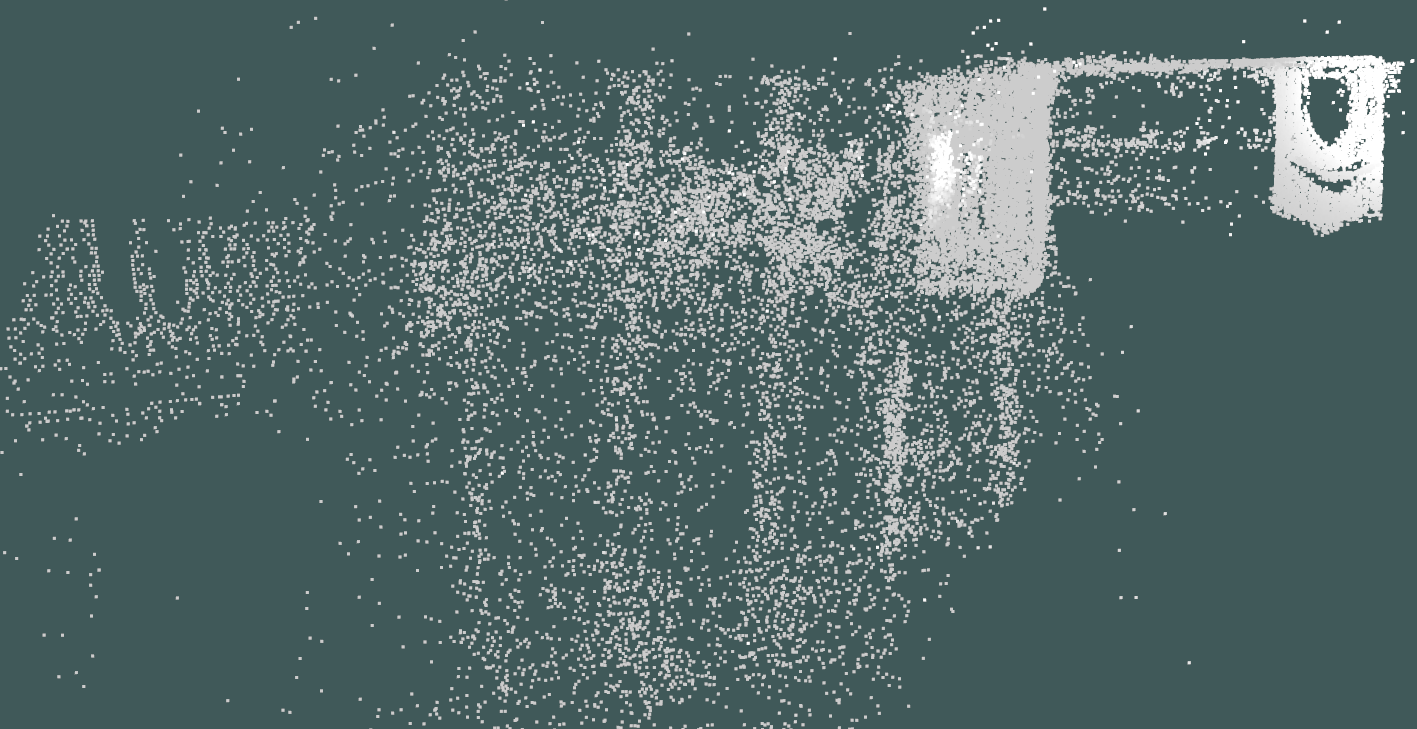
\includegraphics[width=.48\textwidth]{Pictures/cathedral_ceres.png}}~
    \subfloat[HLMDL:Cathedral-46正视图]{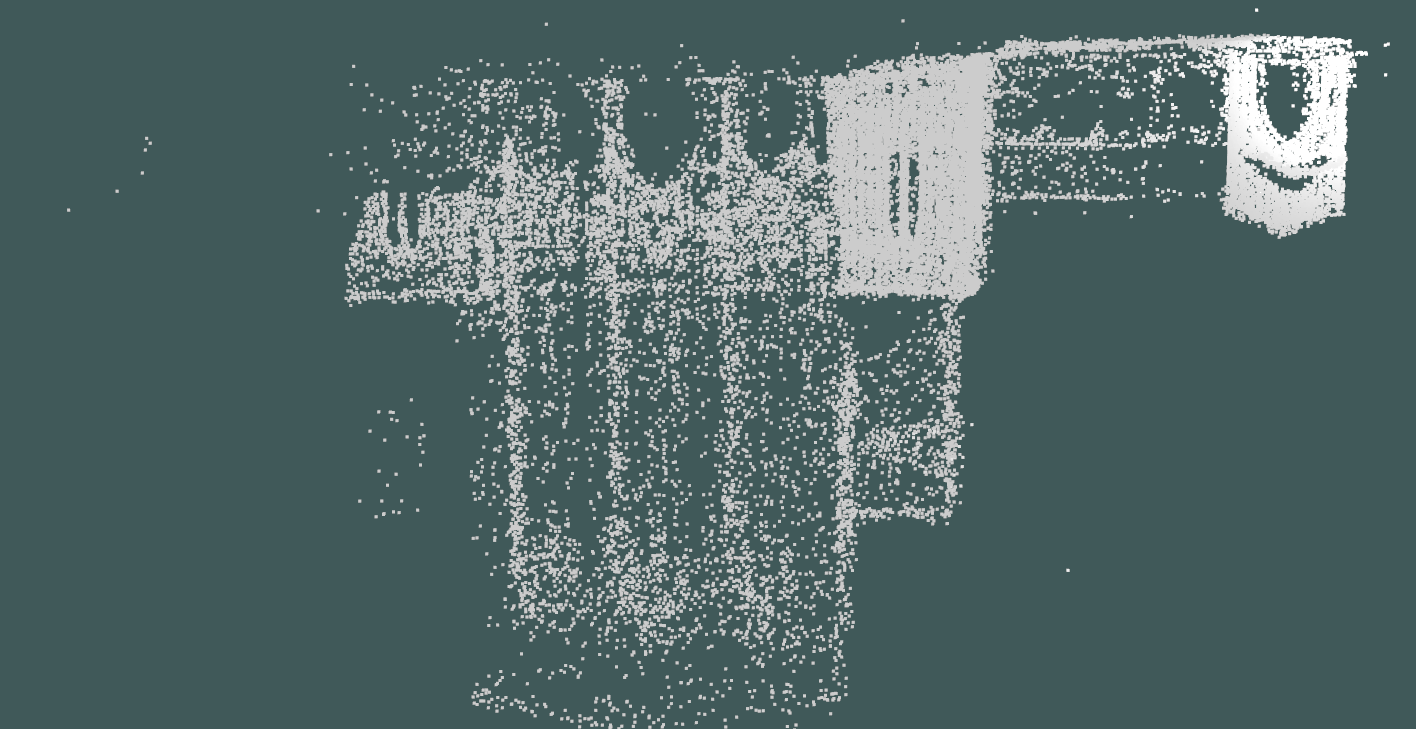
\includegraphics[width=.48\textwidth]{Pictures/cathedral_spec3.png}}
    \\
    \subfloat[Ceres-LM:Cathedral-46俯视图]{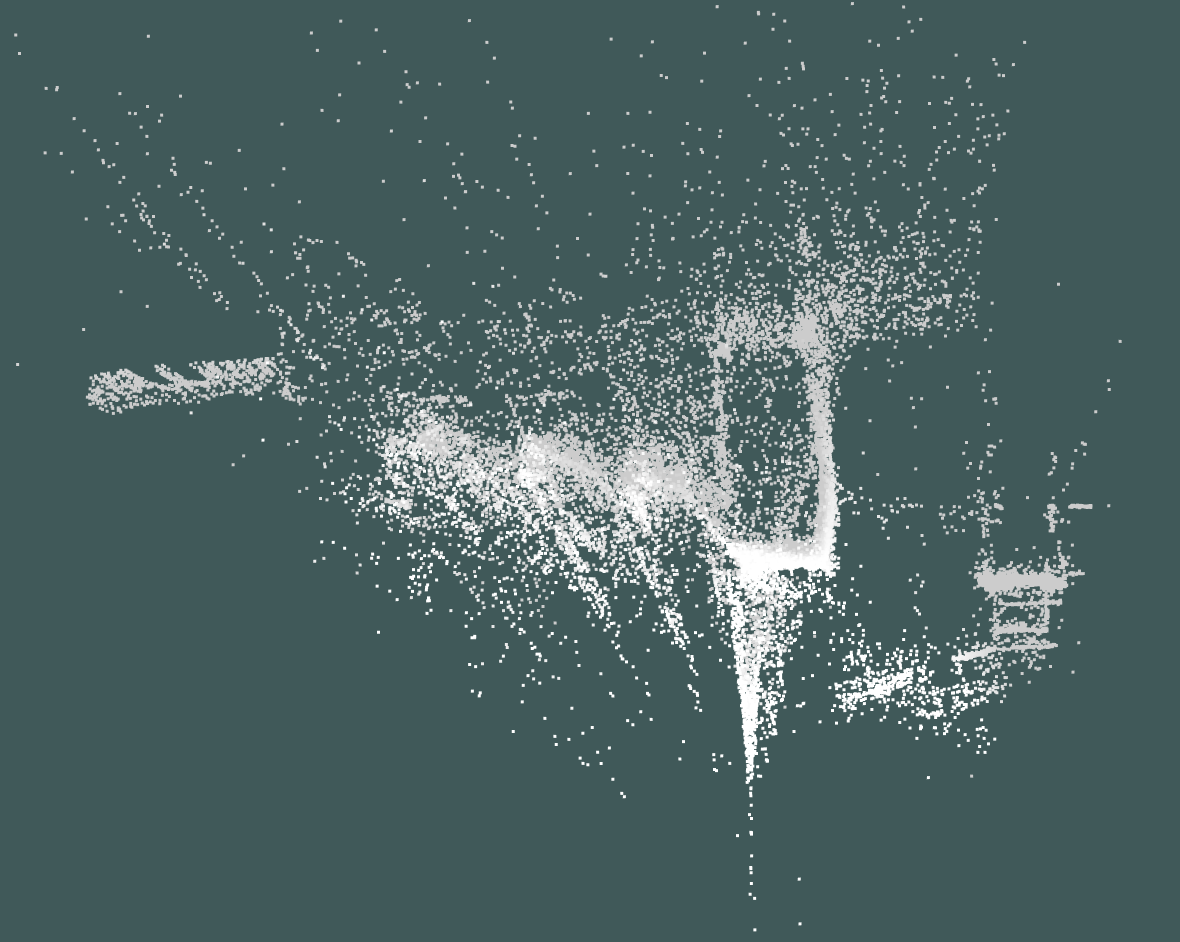
\includegraphics[width=.48\textwidth]{Pictures/cathedral_ceres_up.png}}~
    \subfloat[HLMDL:Cathedral-46俯视图]{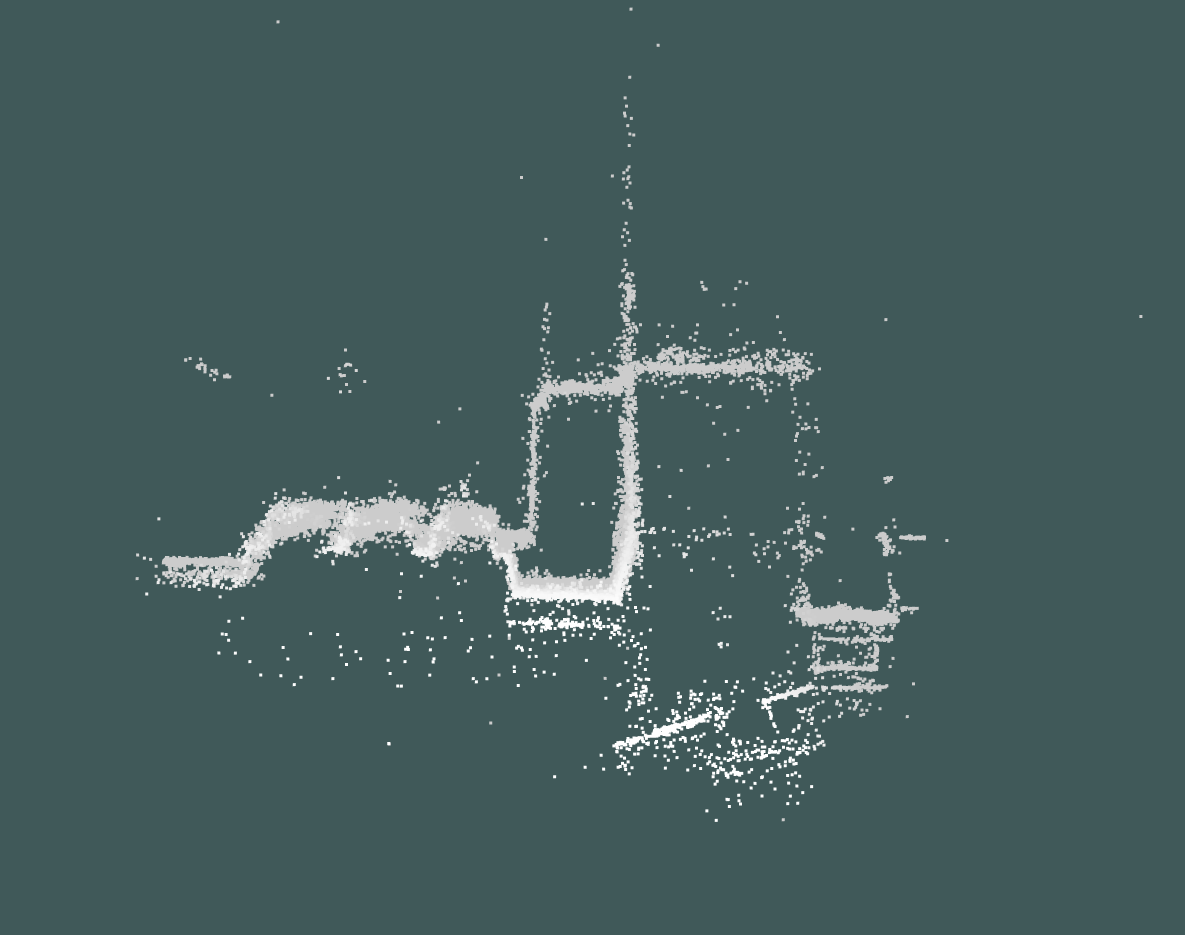
\includegraphics[width=.48\textwidth]{Pictures/cathedral_spec3_up.png}}
    \caption{数据集Cathedral-46运行结果:左列为Ceres-LM求解所得的点云,右列为HLMDL求解所得的点云}
    \label{fig:cathedral}
\end{figure}

综上所述,基于本文提出的增量式集束调整框架无论是在效率还是在精度上都达到了可用的水准。不同的数据集测试结果表示,在精度接近的情况下,本文提出的HLMDL-增量舒尔补算法相对于Ceres-Solver的测试基准,求解时间减少了$84.3\%$至$62.5\%$不等,显著提升了效率。

\section{本章小结}

本章通过求解一般的最小二乘曲线拟合问题,验证了本文提出的集束调整框架的通用性。也通过在模拟VISLAM数据集Cubic-50和开源VSLAM数据集上测试对比了本文提出的增量式舒尔补集束调整优化算法和流行的开源Ceres-Solver的求解效率和精度。得益于高效的增量式舒尔补算法和基于贝叶斯树的PBT回代算法,以及基于块状稀疏矩阵的矩阵计算和存储方式,本文提出的框架达到了较高的求解效率。可以看到在各个数据集上,相比开源的Ceres-Solver,本文提出的基于增量舒尔补的集束调整方法均在保证一定精度的前提下将求解时间减少了$60\%$以上,显著提升了效率。

值得注意的是,本文提出的集束调整框架仍然具有较高的通用性和可扩展性:除了集束调整问题,也可以求解一般的非线性最小二乘问题;除了提供的Cholesky分解法和I-PCG方法,用户也可以自定义新的线性求解方法,以供不同场景使用。
